 \chapter{Network Primitives for DYNAP-SE1}
 \label{appendix:network_primitives}

 This section describes the functionality of the several Python classes that create and control network blocks on the DYNAP-SE1 chip.
 All of these classes require initialization of the Samna backend and work with the \pyobject{model} object returned by it.\\
 
 Every class described later assumes the following block is executed:

 \begin{lstlisting}[language=Python, caption=Initialization of locally connected DYNAP-SE1 board]
import samna
import dynapse1utils as ut

model, _ = ut.open_dynapse1()
\end{lstlisting}

 \section{Clustered WTA class}
 
 This class configures a scalable clustered Winner-take-all (WTA) configuration with the possibility to control hyperparameters such as the connectivity density of specific connection subgroups.\\

\noindent\textbf{Link:} \url{https://code.ini.uzh.ch/dzenn/ctxctl-wta-testbench}\\

 Figure \ref{fig:global_inh_wta_connectivity_labels} shows the full available connectivity profile of the network with hyperparameter label names. Each hyperparameter takes a value from 0 to 1 and defines the connectivity density of the respective group of connections, where 1 is full all-to-all matrix, 0 is no connections at all, and all values in between would results in a random sampling of the fully connected matrix, preserving the same fixed number of pre- and postsynaptic connections for every neuron.

\begin{figure}[h]
    \centering
    \begin{subfigure}{.49\textwidth}
        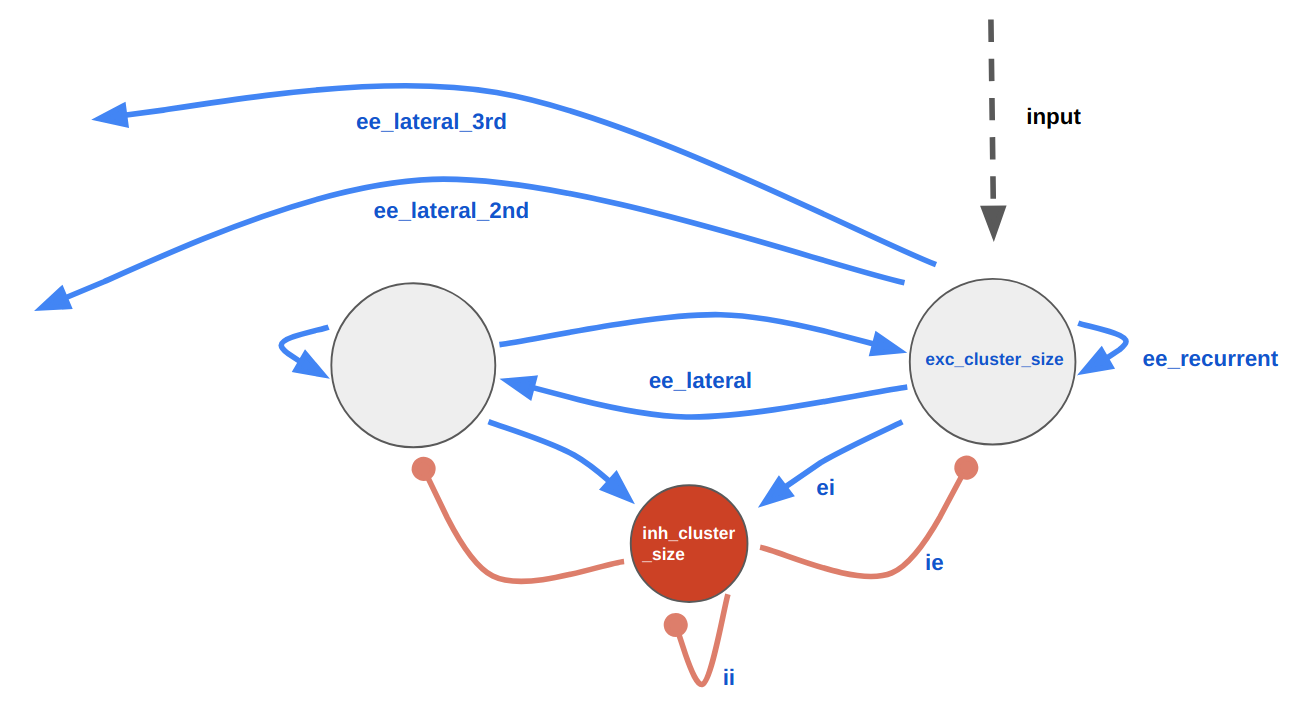
\includegraphics[width=\textwidth]{img/appendices/global_inh_wta_connection_labels.png}
        \caption{Global INH mode}
        \label{fig:global_inh_wta_connectivity_labels}
    \end{subfigure}
    \begin{subfigure}{.49\textwidth}
        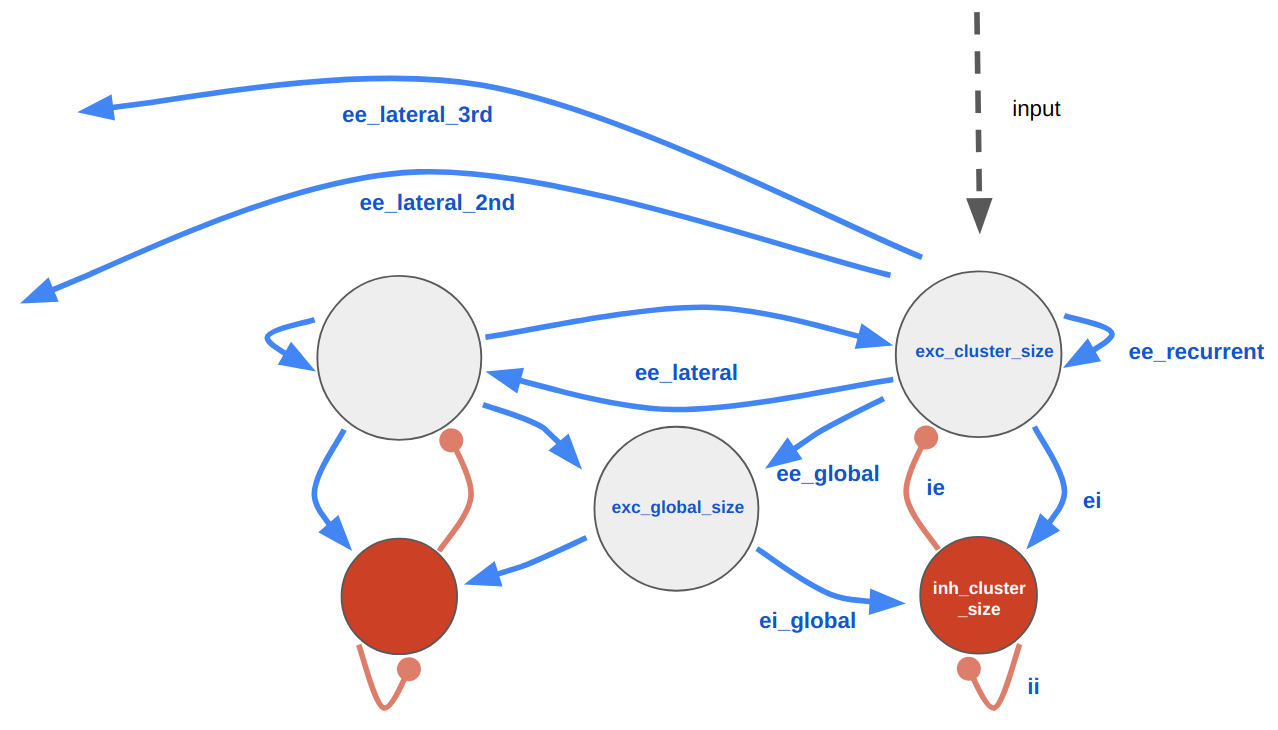
\includegraphics[width=\textwidth]{img/appendices/local_inh_wta_connection_labels.png}
        \caption{Global EXC mode}
        \label{fig:local_inh_wta_connectivity_labels}
    \end{subfigure}
    \caption[Illustration for the label names of the groups of connections of the WTA class]{Illustration for the label names of the groups of connections of the WTA class for the case of global inhibitory and excitatory populations used in the configuration dictionary.}
    \label{fig:local_inh_wta_connectivity_labels}
\end{figure}

 Before sampling is done, the calculation of the integer number of connections each neuron would send and receive is done by deterministically rounding down the result of the multiplication of the connectivity probability and the respective presynaptic population size, thus keeping the overall fan-in of every neuron of the group constant.

\begin{lstlisting}[language=Python, caption=WTA structure connectivity hyperparameters]
exc_cluster_size=8
exc_size=16
inh_size=8
inh_cluster_size=4

connectivity={'wta_structure': 'global_exc',
                'ee_recurrent': 1.0,
                'ee_lateral':0.0,
                'ee_lateral_2nd':0.0,
                'ee_lateral_3rd':0.0,
                'ei': 1.0,
                'ie': 1.0,
                'ii': 0.8,
                'ee_global':0.4,
                'ei_global':0.5,
                'exc_global_size': 8}
\end{lstlisting}

\subsection{Internal variables}

\dz{TODO: Finish the class description}\\

\noindent The class provides access to the network's internal substructures:

\begin{itemize}
    \item \verb|rates| is the array of rates for the neurons 
    \item \verb|exc_population|
    \item \verb|exc_population_ids|
    \item \verb|inh_population|
    \item \verb|inh_population_ids|
    \item \verb|sink_node|
    \item \verb|running_raster_sink_node|
    \item \verb|poisson_spike_gen|
    \item \verb|net_gen|
    \item \verb|expected_value|
    \item \verb|estimated_value|
\end{itemize}


\subsection{Class methods}

After the instantiation of a \pyobject{WTA} network object, an interaction with the created network is allowed.\\

\noindent\textbf{Reading events, extracting population codes}\\

Function \verb|get_rates(self, measurement_period = 1, spike_limit = None, keep_buffer=False, return_spikes=False, debug=False)| records events from the specified neurons for the duration of the \verb|measurment_period|.

\begin{itemize}
    \item \verb|get_rates()| is the array of rates for the neurons 
    \item \verb|set_bump_input()|
    \item \verb|set_regular_bump_input()|
    \item \verb|set_double_bump_input()|
    \item \verb|set_square_input()|
    \item \verb|set_freq_input()|
    \item \verb|set_single_neuron_input()|
    \item \verb|set_dc_input()|
    \item \verb|set_preloaded_stimulus(self, spike_train, verbose=False)|
\end{itemize}
 
\subsection{Initialization}

\begin{lstlisting}[language=Python, caption=Initialization of the WTA network with a global inhibitory cluster]
#%% Global INH 16 clusters, soft WTA

start_neuron=16
exc_size=128

chip_id=1
core_id=0
mode='clustered_WTA'
exc_cluster_size=8
inh_cluster_size=4

inh_size=20
connectivity={'wta_structure': 'global_inh',
                'ee_recurrent': 0.8,
                'ee_lateral':0.5,
                'ee_lateral_2nd':0.0,
                'ee_lateral_3rd':0.0,
                'ei': 0.2,
                'ie': 0.2,
                'ii': 0.0,
                'ee_global':0.0,
                'ei_global':0.0,
                'exc_global_size': 0}


input_multiplier=5
clustered_input=True
allow_self_exc=False
debug=True

TG = DynapseTestGroup(model, start_neuron,exc_size,inh_size,chip_id,core_id,mode,core_id+1, None, exc_cluster_size,inh_cluster_size,connectivity,input_multiplier,clustered_input,allow_self_exc,debug=debug)

\end{lstlisting}

\subsection{Providing input to the network}

\subsection{Reading the output}

\subsection{Supplementary functions}

\begin{itemize}
    \item \verb|double2pop_code(inputSize, sigma=None, amplitude=100)| is the array of rates for the neurons 
    \item \verb|pop_code2double(rates)|
\end{itemize}

%\newpage
%\section{Delay chain/Oscillator}

%\newpage
%\section{Threeway relational network}

%This class combines all of the above-mentioned and provides a scalable set of delay chains within the selected core.
 